%%%%% METHODS %%%%%

\begin{figure*}[htbp]
    \centering
    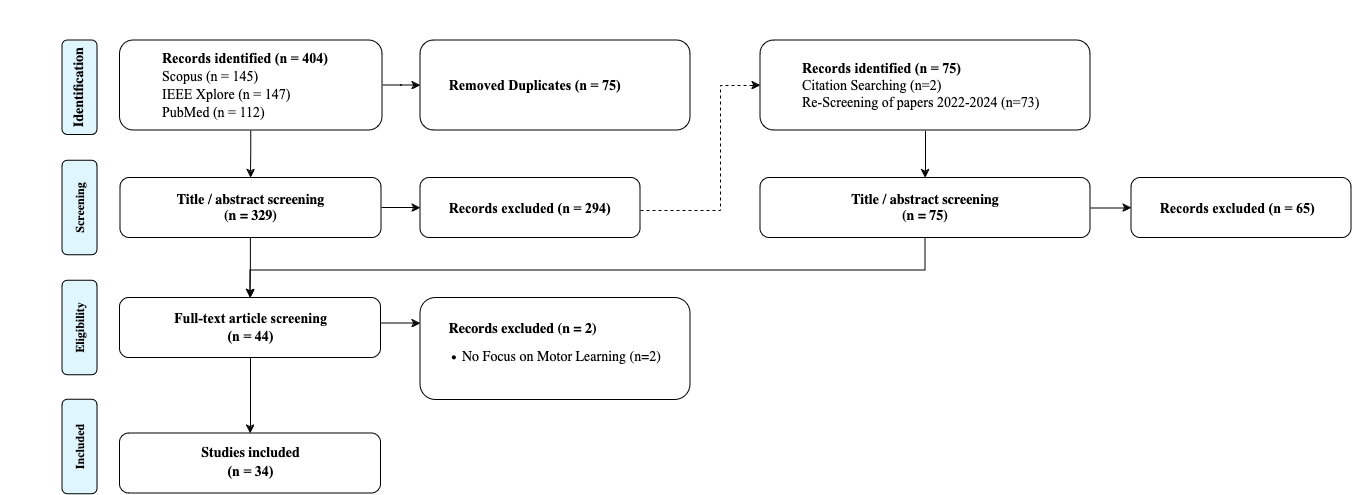
\includegraphics[width=\linewidth]{figures/prisma_overview.png} 
    \caption{Overview of the methodology using the PRISMA method}
    \label{fig:prisma}
\end{figure*} 

\section{Methods}
\label{sec:methods}

The method of the systematic review was based on the PRISMA methodology \cite{Page2021TheReviews} to ensure transparent and complete reporting on the topics examined.

\subsection{Search Strategy and Eligibility Criteria}
\label{sec:eligibility}
Several relevant articles were reviewed at the beginning to find eligible search terms. The query based on the research question consists of three main parts, namely \textit{virtual reality}, \textit{somatosensory feedback}, and \textit{motor learning}, each term with their respective synonyms. 

The final search query was as follows: motor AND (learning OR control OR training OR skills) AND (((virtual OR augmented) AND reality) OR ((remote OR virtual OR simulated) AND environment)) AND (((somatosensory OR haptic OR tactile OR proprioceptive OR kinesthetic OR cutaneous OR somatic) AND 
(cue* OR feedback OR rendering OR stimul*)) AND (fidelity OR realism OR accuracy OR precision OR exactness OR specificity)). The search terms were applied for the article title, abstract, and keywords.

Three databases (Scopus, IEEE Xplore, and PubMed) were searched in April 2024. Based on the required syntax of each database, the search query was slightly adapted. For example, as PubMed only allows for the use of an asterisk for words containing more than three letters, the term \textit{cue*} was changed to (\textit{cue} OR \textit{cues}). The exact search queries can be found in \ref{sec:queries}. 

To qualify for inclusion, studies had to focus on the impact of somatosensory feedback on motor learning in humans. We included studies with healthy participants only, as patients often know how to perform a movement but are physically constrained by their condition, therefore augmented feedback may help the motor learning of patients in a different way compared to healthy subjects \cite{Sigrist2013AugmentedReview}. There were no publication date or language limits.

Conversely, studies were excluded if they (i) did not relate to motor learning in humans; (ii) focused on systems not providing haptic feedback in VR; (iii) were concerned with a neurological condition affecting motor learning; or (iv) explained a new assessment system for the evaluation of motor learning.

\subsection{Study Selection}
At first, duplicate publications were identified and removed. The results were then screened based on their title and abstract. 

In this review, we wanted to emphasize more recent studies to reflect the significant impact of recent technological advances in VR on the field. Therefore, records published in the years 2022-2024 were re-screened and also included in the further process, if they were only partially fitting the eligibility criteria. Additional papers were identified using citation searching.

Finally, the full-text articles were assessed to determine their eligibility for inclusion in the review (see fig. \ref{fig:prisma}).


\section{Search Results}

%%%% Rewrite for precise numbers!! %%%%%

The search yielded 404 results, which were saved in the library of Mendeley. 75 duplicates were found and removed. The remaining 329 records were screened based on title and abstract first. This led to the preliminary exclusion of 290 records, of which 73 records were re-screened as they were from the years 2022-2024 (see fig. \ref{fig:prisma}), along with 3 papers that had been included based on citation search. 
65 records were excluded during this screening.

In total, 50 articles were eligible for the full-text screening. Of these, 14 were excluded based on the exclusion criteria, and the remaining 36 studies were included in this review.


\subsection{Study characteristics}
\subsubsection{Year of publication}
The year of publication of the included studies ranges from 2000 to 2024. As seen in \ref{fig:years}, the number of studies has greatly increased in the past decade, with a peak in 2018.

\begin{figure}[htbp]
    \centering
    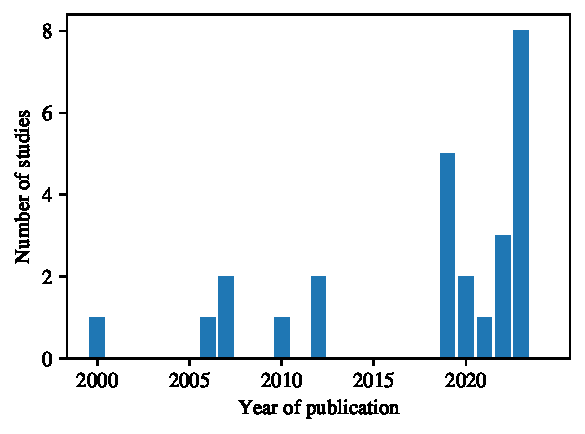
\includegraphics[width=\columnwidth]{figures/years.pdf} 
    \caption{Publication dates of the included articles}
    \label{fig:years}
\end{figure} 


\subsubsection{Body parts involved}
\note{
\begin{itemize}
    \item Graph to quantify involved body parts (pie chart)
\end{itemize}
}

\section{Definitions}
\subsection{Feedback Fidelity}

Feedback fidelity refers to the accuracy and realism of stimuli provided to the user when they are interacting with the virtual environment. 

Several frameworks have been proposed to assess the feedback fidelity of the VE. They concentrate on either the physical attributes of the system (e.g. the FIFA framework developed by McMahan et al. \cite{McMahan2011ExploringGames}), aim to evaluate feedback fidelity through questionnaires (e.g. the haptics addition \cite{Boos2017ErweiterungHaptik} to the User Experience Questionnaire \cite{Laugwitz2008ConstructionQuestionnaire}) or focus on the effect of the system. Huang et al. for example suggested that skill transfer might be a useful paradigm to evaluate the level of fidelity, assuming that if an environment has infinite fidelity and is therefore perfectly recreating the sensations of the real environment, then there would be no performance loss when transferring the skill from the virtual to the real environment \cite{Huang2006}.

These frameworks, while addressing particular subjective and objective dimensions of haptic feedback systems, fail to capture their full diversity. This gap is addressed by Muender et al., who developed the Haptic Feedback Fidelity Framework \cite{Muender2022HapticReality}.
It helps to evaluate a system's haptic feedback fidelity ranging from abstract to realistic and introduces versatility as a second axis, which allows for the differentiation between generic and specific haptic feedback systems. 

In this review paper, we extend the Haptic Feedback Fidelity Framework by a third axis, taking into account a quality score for each haptic feedback system. This score determines how many of the parameters assessed in the framework have actually been provided by the researchers. Furthermore, single aspects of the framework are extended in an attempt to make the evaluation more transparent and quantifiable. 


We then evaluate the selected articles described in section \ref{sec:methods}  based on this framework. This will help to create a dataset with transparent methods to overcome the sometimes opaque classification of haptic fidelity by researchers, that base the level of fidelity on few or no factors at all (e.g. \cite{Grant2019}). 


\section{Framework}

The framework is built on eight foundational factors, describing the features of a system and their value, and six limiting factors that negatively impact the perception. Each factor is rated on a 5-point Likert scale (0-4). We are aiming to briefly explain the framework by Muender et al. and describe our small adaptions to make the factors easier to quantify. For more details and examples we would therefore like to refer to the Haptic Fidelity Framework \cite{Muender2022HapticReality}.

We developed equation \ref{eq:diff}, which can help with quantifying the factors, with $RE$ standing for the quantity or area in the natural occurrence:

\begin{equation}    
4 \cdot \left(1 - \left(\frac{\left|VR_{\text{factor}} - RE_{\text{factor}}\right|}{RE_{\text{factor}}}\right)\right)
\label{eq:diff}
\end{equation}


\subsection{Haptic Fidelity}
\subsubsection{Foundational Factors}
\paragraph{Body Location}

This factor describes whether the haptic feedback on the user's body created by the system aligns with where the person would perceive the stimulus in the natural occurrence of the intended haptics \cite{Muender2022HapticReality}. Here, the ability to localize a point on the skin for different body parts is taken into account, giving more weight to body parts where the point localization threshold is significantly lower (e.g. hallux, upper lip, nose, cheek, forehead, and all fingers) \cite{Lederman2009HapticTutorial}.

\paragraph{Body Area} 
This factor accounts for the degree to which the same extent of the body surface of the user is involved in the simulation compared to the natural occurrence of the intended haptics. The density of mechanoreceptors should be considered \cite{Muender2022HapticReality, Lederman2009HapticTutorial}.

\paragraph{Stimuli}
This factor quantifies the degree to which the same haptic receptors of the user are involved. The table provided by Muender et al. can help in distinguishing which haptic stimuli are affected by which physical property of the handled object or the VE \cite{Muender2022HapticReality}.

\paragraph{Magnitude}
The magnitude describes to which degree the system can create the same strength (e.g. force) or variation (e.g. texture) of haptic stimuli compared to the natural occurrence of the intended haptics \cite{Muender2022HapticReality}. While some researchers state that high-fidelity haptic devices can typically provide up to 40N of force \cite{Grant2019}, we argue that the necessity to provide a certain magnitude of force highly depends on the stimulated body parts and the task itself. While a magnitude of 9 N, as provided by for example the Novint Falcon haptic device, might be sufficient for manipulating light objects with the fingers, it will arguably not be enough to mimic a ballistic movement with the entire arm handling heavy objects.
If magnitude and variation can be fully matched by the system, it would receive 4 points for this factor. If only magnitude or variation are matched, this would result in a score of 2.

\paragraph{Sensory Integrity}
This factor determines whether the haptic stimuli created medium that is used for stimulation matches with the perception of the other senses and is in line with the intent \cite{Muender2022HapticReality}. For example, Zenner et al. use actuated flamenco fans to mimic the perception of weight by leveraging the drag created through the air resistance \cite{Zenner2019}. This can be rated with a medium degree of integrity, as it does not match the feeling of weight exactly, but it is superior to no weight perception or flamenco fans without actuators. 

\paragraph{Degrees of Freedom}
This factor describes if the system can provide haptic feedback in the same number of degrees of freedom (DoF) as in the natural occurrence of the intended haptics \cite{Muender2022HapticReality}. In case of the tank gunnery simulation for example, in which haptic feedback was introduced by \cite{LiuG2014}, providing haptic feedback in the two rotational axes would be sufficient, as the interface for controlling the gun also only has two DoF.

\paragraph{Hardware Precision}
This factor is determined by the extent to which the system can reproduce the detail of haptic feedback compared to the natural occurrence of the intended haptics \cite{Muender2022HapticReality}. 
It is influenced by the accuracy of the system (e.g. encoder resolution of stepper motors) and the refresh rate of the haptic stimulation as well as the display. According to Coles et al., the commonly accepted refresh rate to provide realistic force feedback is at around 1,000 Hz \cite{Coles2011TheArt}, although depending on the object's stiffness. Coles et al. states that hard objects require higher refresh rate than soft objects. Although we agree with this terminus, we suggest that also the type of task has to be taken into account when evaluating hardware precision. Fast and precise tasks such as following a 3D path with a ring in the shortest possible time \cite{Oquendo2024} require a higher feedback frequency than controlling an underwater robot through currents with moderate speed and predictable obstacles \cite{Xia2023}.

For this review, we give a perfect score for a system with 1,000 Hz refresh rate for the haptics regardless on the task and then depending on the task and the object stiffness give fewer points to the system if the refresh rate is lower.

Regarding the accuracy of the haptic feedback, the human ability to localize a point on the skin needs to be considered, as feedback has to be more precise when applied to sensitive areas such as the finger tips compared to less sensitive areas such as the shoulder \cite{Lederman2009HapticTutorial}.

Regarding the display frequency, according to Lim et al. an update rate of 30 Hz is required for the display to be realistic \cite{Lim2021}, whereas Han et al. found that there was a great increase for frequencies up to 120 Hz in motion perception. This is especially important when objects are moving quickly, or the visual perception of ones own body parts is important for the task \cite{Han2022AssessingPotentials}.
We therefore give a perfect score if the display frequency is 120 Hz, and reduce it if the display frequency is lower and the task requires fast moti
The positive effect of refresh rate is most significant when the refresh rate is increased from 60 to 120 Hz, and then the positive effect gradually gets into the realms of diminishing returns as the refresh rate range continues to increase above 120 Hz. This trend has no concern with the form of motion stimulation.

\begin{comment}
"The required refresh rate to provide realistic
force feedback is commonly accepted to be at least 1,000 Hz.
However, this refresh rate is widely debated. According to
Burdea [14], a minimum refresh rate of only 300 Hz is
acceptable. Conversely, a study by Booth et al. [15] using
SensAble’s Premium 1.5 to deduce the minimum acceptable
haptic refresh rate, suggests that “a minimum acceptable
refresh rate must lie within the 550-600 Hz range.” The
necessary rate of update is dependent upon the stiffness of
the surfaces to be simulated. A stiff contact between objects is
better simulated by higher refresh rates, whereas lower
refresh rates are satisfactory for softer objects. Additional
methods can be applied to simulate touching stiffer objects
such as combining vibrations with force to the end effector to
represent the small vibrations felt upon object contact [16].
Typically, a trade-off must be made between the accuracy of
the haptics effects produced and the speed required within
the application." \cite{Coles2011TheArt}
About latency and its impacts: \cite{Gourishetti2018PassiveFeedback}.
Ballistic movements: rapid, involuntary movement which is motor programmed, and for which visual feedback is not possible \cite{Wall2000}.
\end{comment}

\paragraph{Software Precision}
This factor describes the detail to which the software can simulate the intended haptic feedback. This concerns for example the exactness of collision boxes in the software \cite{Muender2022HapticReality}

\subsubsection{Limiting Factors}
\paragraph{Dependency}
The factor dependency measures to which degree the absence of different dependent haptic stimuli that are usually perceived together, in reality, has an impact on the haptic perception of the system. For more details see \cite{Muender2022HapticReality}.

\paragraph{Distinguishability}
This factor describes if different physical properties in the VE can be distinguished by the haptic feedback the system provides. If the system for example only gives vibrotactile feedback when manipulating an object, this would increase the score of this limiting factor, as different properties of the object such as weight or texture cannot be distinguished. 

\paragraph{Hardware Latency}
The delay between the interaction with the object in the VE and the haptic stimulation by the system determines this factor. While a latency of up to 25ms has been shown to not affect the user, delays greater than 25ms can have a noticeable impact on performance \cite{Muender2022HapticReality}.

\paragraph{Software Latency}
The same threshold as for hardware latency also applies to this factor, which is concerned with the software latency's impact on the system's haptic perception.

\paragraph{Side Effects}
Haptic systems can produce unintended haptic stimuli such as vibration or friction. This factor describes how these side effects influence the haptic perception of the system. 

\paragraph{Constraints}
This factor describes the degree to which the system constrains the user's movement other than in the intended way \cite{Muender2022HapticReality}.

\subsubsection{Scoring}

The score for the haptic fidelity is calculated based on equation \ref{eq:fidelity_score}, in which $X_F$ are the foundational and $X_L$ are the limiting factors \cite{Muender2022HapticReality}:

\begin{equation}
	\frac{\sum_{N_F}^{0} X_F}{N_F} \cdot e^{-0.0027 \left(\sum_{N_L}^{0} X_F^2 \right)^2}
	\label{eq:fidelity_score}
\end{equation}

\subsection{Versatility}
The versatility is assessed on a 5-point Likert scale with 0 for very specific system that can only be used for one scenario, and 4 for systems that can produce very generic haptic feedback. For the classification, we follow the example categories provided by Muender et al. \cite{Muender2022HapticReality}.


\subsection{Quality score}
\label{sec:quality}
In total, 14 parameters needed to be evaluated for each haptic feedback system. We calculated a score based on the percentage of factors, that were not described in the paper itself, nor could be accessed through internet research (e.g. by looking up the specifications for the commercial products).
We divided the papers into four quality groups based on the quality score :

\begin{enumerate}
	\item High quality: $q > 0.9$
	\item Good quality: $0.8 < q \leq 0.9$
	\item Medium quality: $0.7 < q \leq 0.8$
	\item Low quality: $q \leq 0.7$
\end{enumerate}